%=====================================================================
\section{Improving the models}\label{sec:improve}
%=====================================================================
After the baseline experiments we tested a series of improvements, \textbf{one change at a time} so that
the effect of each can be measured. Ideas came from the EDA, from the Grad-CAM analysis, from the literature and
from team discussion. As before, \textbf{every choice is made on the validation set}; the test set is only
reported. All runs in this section use a higher-resolution image cache (shorter side 512\,px instead of 256\,px).
This alone changes results slightly: the standard ResNet-50 recipe re-run on the new cache scored 83.8\% instead of
82.4\% (sharper crops when RandomResizedCrop zooms in, plus run-to-run noise). We therefore compare
\emph{within} each series and always include a re-run baseline.

%---------------------------------------------------------------------
\subsection{Bird-crop preprocessing (bounding boxes)}
\textbf{Motivation.} The bird covers only \textbf{32\% of the image} on median (as little as 5\%; 2,739 images are under
20\%, Fig.~\ref{fig:birdcrop}), so about two-thirds of every input is background (branches, water, feeders). Grad-CAM had
already shown that the scratch CNN used the red feeder rather than the hummingbird --- a background shortcut.

\textbf{Method.} The Hugging Face version of CUB has no annotations, so we extracted the official bounding boxes
(\texttt{bounding\_boxes.txt}) from the original CUB-200-2011 release once and matched them to all 11,788 images by file name
(\texttt{resources/cub\_bounding\_boxes.csv}). Each image is cropped to a \emph{square} box around the bird with a 15\% margin on
every side (\texttt{crop\_to\_bird} in \texttt{src/data/datasets.py}), so that the later centre crop does not cut off tails or
wings, and some context remains. The crop is applied identically to train, validation and test images; all other preprocessing
and augmentation then run on the cropped image.

\begin{figure}[H]\centering
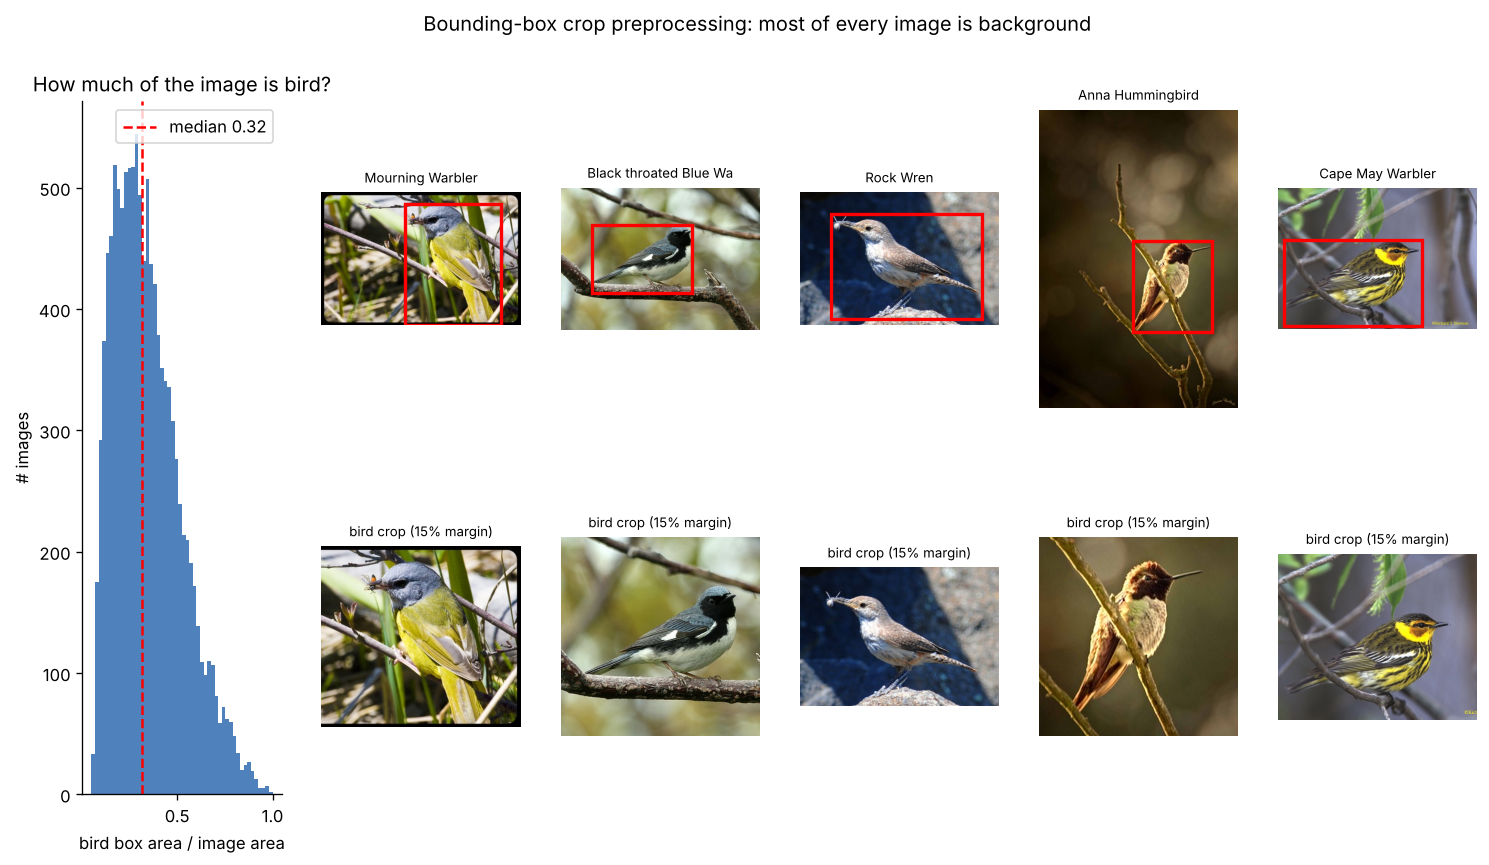
\includegraphics[width=\linewidth]{figs/14_bird_crop.png}
\caption{Left: fraction of the image covered by the bird. Right: original images with the official box (top) and our crop (bottom).}\label{fig:birdcrop}
\end{figure}

\textbf{Results.} Cropping is the single most effective change: \textbf{+6.3 points} for the scratch CNN (52.5\%$\rightarrow$58.7\%)
and \textbf{+1.3 points} for ConvNeXt-Tiny (84.6\%$\rightarrow$85.9\%). It helps the scratch CNN much more because a network that
learns from 5,400 images cannot afford to spend capacity on background, while ImageNet features already ignore much of it.
Cropping also acts as a \emph{zoom}: the bird occupies the whole $224\times224$ input, so field marks get about $3\times$ more pixels.

\textbf{Caveat (fairness).} Using the ground-truth box \emph{at test time} uses an annotation that a real user would not provide.
These results are therefore reported separately as ``with ground-truth boxes'' and are not compared with annotation-free methods;
we also report our best \emph{full-image} model. In a deployed system (and for Milestone~2) a bird detector would supply the box.

%---------------------------------------------------------------------
\subsection{Resolution}
At 384\,px (instead of 224) on full images, ConvNeXt reached a higher validation accuracy (85.1\% vs.\ 84.3\%) but the same test
accuracy (84.6\%); its best epoch came early (14 of 30) and it costs $2.3\times$ more time per epoch. With the bird crop, 384\,px
added +0.3 points (85.9\%$\rightarrow$86.2\%). \textbf{Conclusion:} at our budget, cropping is a cheaper and more effective
``zoom'' than raising the resolution of the whole image; the two partly do the same thing.

%---------------------------------------------------------------------
\subsection{Augmentation ablation}
Seven augmentation strategies were compared on the same model (ResNet-50 fine-tune, full image, 224\,px, 30 epochs):

\begin{figure}[H]\centering
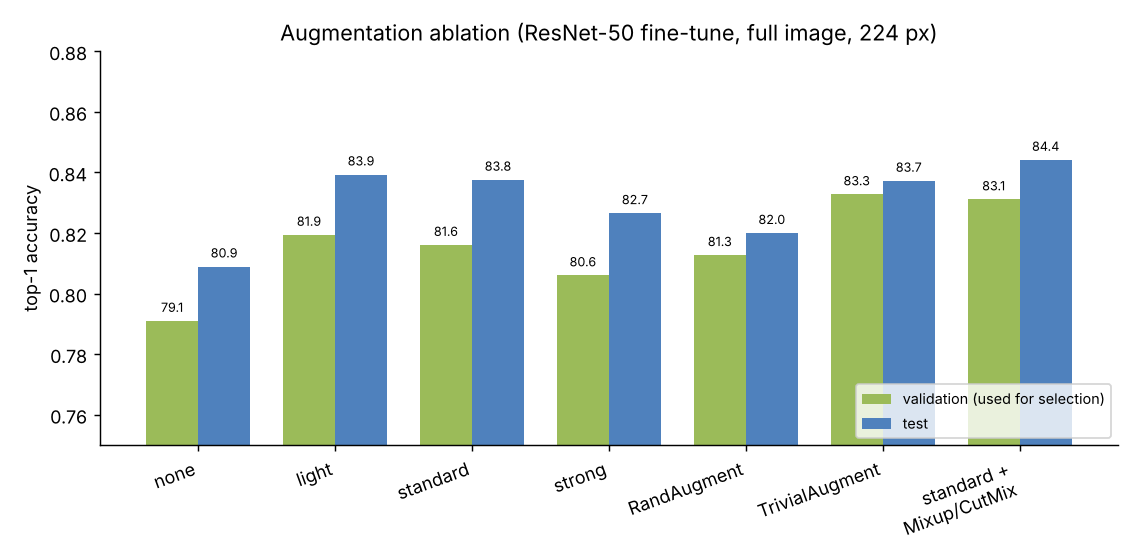
\includegraphics[width=0.85\linewidth]{figs/ablation_aug.png}
\caption{Augmentation ablation: validation (selection) and test accuracy.}\label{fig:augabl}
\end{figure}

\begin{itemize}
\item \textbf{Augmentation matters}: with none, test accuracy is 80.9\%; every geometric augmentation improves it by about 2--3 points.
\item \textbf{Light $\approx$ standard} (83.9\% vs.\ 83.8\%, within noise).
\item \textbf{Too strong hurts}: \emph{strong} (82.7\%) sometimes crops the bird out entirely (Fig.~\ref{fig:aug}).
\item \textbf{RandAugment is the worst augmented setting (82.0\%)}. Its policy includes colour-changing operations (Color, Solarize,
Posterize, Equalize). This supports our EDA-based decision not to alter colours: colour is a label-relevant feature for birds.
TrivialAugment, whose operations are sampled with random strength (often weak), stays at the standard level (83.7\%).
\item \textbf{Mixup/CutMix on top of standard is the best} (84.4\% test, 85.0\% with TTA). Mixup blends two images and their labels;
CutMix pastes a patch of one image into another and mixes the labels by area. Both prevent the model from becoming over-confident on
27 images per class. (The low ``train accuracy'' of mixed runs, $\sim$67\%, is measured on the mixed images and is expected.)
\end{itemize}

%---------------------------------------------------------------------
\subsection{Loss function: cosine loss vs.\ cross-entropy}
Cross-entropy keeps pushing the true-class logit up, so on a tiny dataset the network can reduce the loss simply by
\emph{scaling up} its outputs. The cosine loss of Barz \& Denzler~\cite{cosine}, proposed for small datasets trained from scratch,
L2-normalises the output vector and maximises its cosine similarity with the one-hot vector of the true class, so only the
\emph{direction} of the output matters. We implemented their combined form, cosine loss $+\,0.1\times$ cross-entropy on the
normalised vector (\texttt{src/training/losses.py}); predictions use the (scaled) cosine similarities.

\begin{figure}[H]\centering
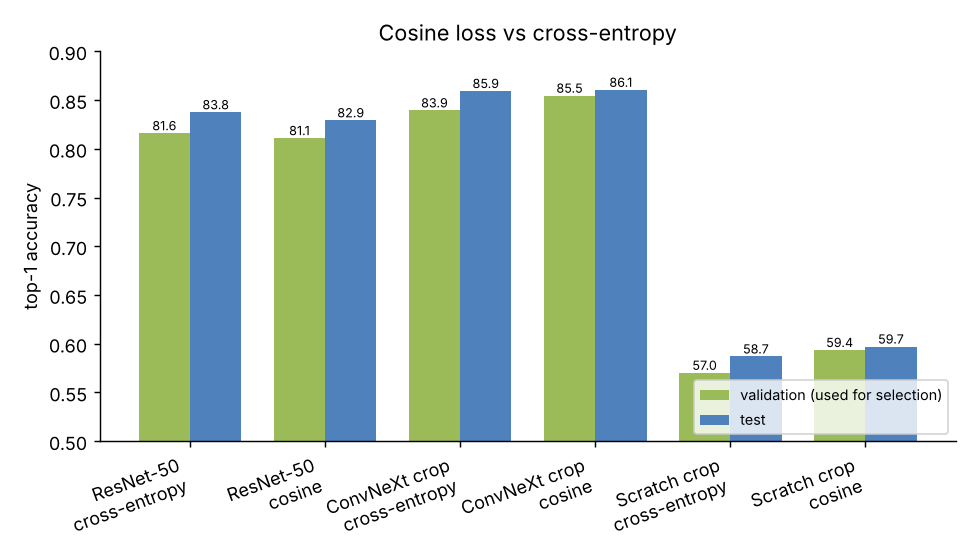
\includegraphics[width=0.85\linewidth]{figs/loss_compare.png}
\caption{Cosine loss vs.\ cross-entropy for three models.}\label{fig:loss}
\end{figure}

\textbf{Results.} As the paper predicts, the cosine loss helps most when training \textbf{from scratch} (+1.0 test, +2.3 validation).
For the pretrained ConvNeXt it improved validation accuracy by 1.5 points (the best single-change validation score, 85.5\%) but test
accuracy only by 0.1; for ResNet-50 it was 0.8 points \emph{worse} on test. With pretrained features the over-confidence problem the
cosine loss addresses is smaller, so its benefit is inconsistent.

%---------------------------------------------------------------------
\subsection{Scratch CNN: combining the improvements}
\begin{figure}[H]\centering
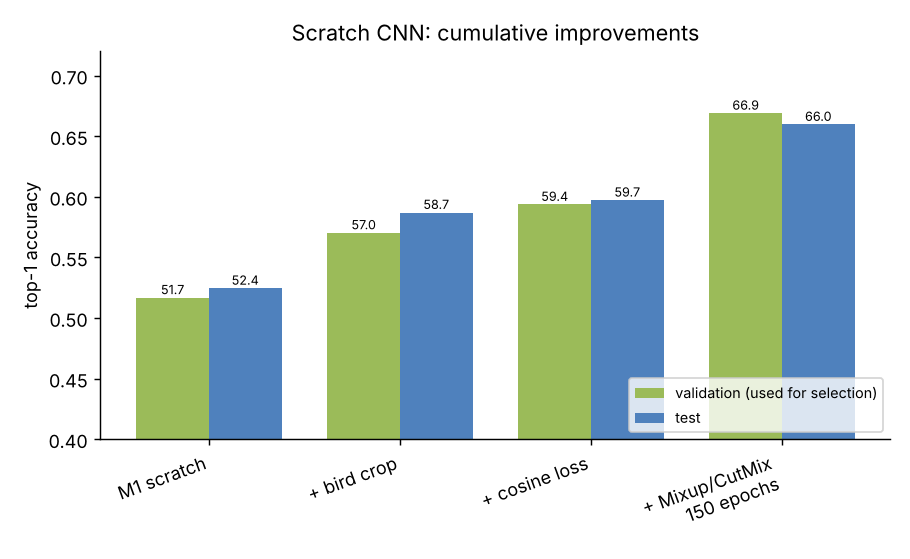
\includegraphics[width=0.7\linewidth]{figs/improve_scratch.png}
\caption{Cumulative improvements of our from-scratch CNN.}
\end{figure}
Bird crop (+6.3), cosine loss (+1.0), then Mixup/CutMix with longer training (150 epochs, +6.2) raised the scratch CNN from
52.5\% to \textbf{66.0\%} (66.6\% with TTA), a gain of 13.5 points without any pretraining. The overfitting gap also shrank: the original
model reached 96\% training accuracy against 51\% validation; with mixing the model can no longer memorise individual images.
Validation accuracy was still rising at epoch 147 of 150, so a longer run is included in the final experiments.

%---------------------------------------------------------------------
\subsection{Test-time augmentation (TTA)}
At test time each image is also classified mirrored (horizontal flip) and the two probability vectors are averaged. TTA improved
\textbf{all 16 runs}, by +0.58 points on average (range +0.22 to +1.07), at the cost of a second forward pass. Being free of training,
it is reported for every run from now on.

%---------------------------------------------------------------------
\subsection{Hyper-parameter tuning v2}
Tuning v1 had one clear limitation: the 8-epoch proxy runs favoured fast-converging settings, and the tuned configuration did not beat
the default at 30 epochs. Tuning v2 fixes the protocol: (i) a 15-epoch proxy, (ii) on the final model family (ConvNeXt-T + bird crop)
rather than ResNet-50, and (iii) four hyper-parameters --- head LR, \textbf{backbone LR multiplier}, weight decay, label smoothing ---
with random search (8 trials).

\begin{figure}[H]\centering
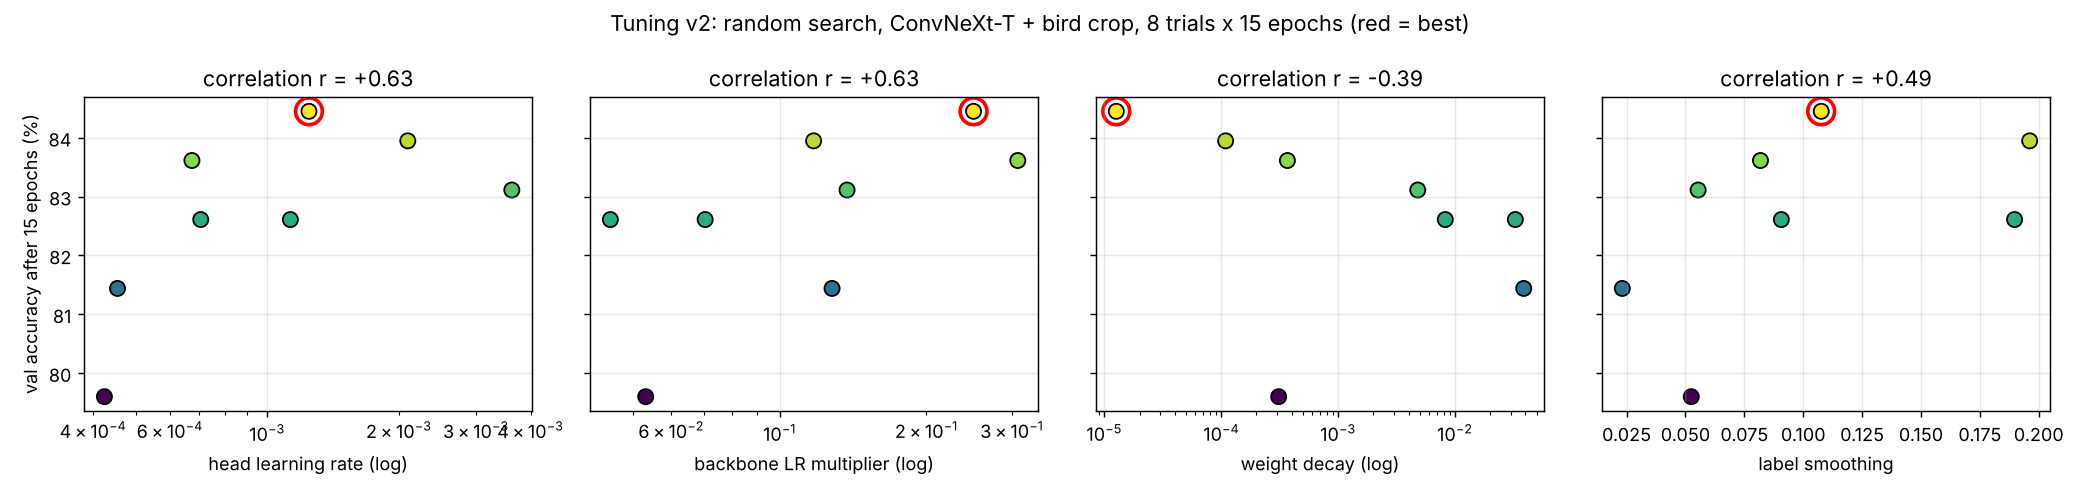
\includegraphics[width=\linewidth]{figs/tuning_v2_params.png}
\caption{Tuning v2: validation accuracy of each trial against each hyper-parameter (red circle = best trial).}\label{fig:tunev2}
\end{figure}

The best trial reached 84.5\% validation accuracy after only 15 epochs (head LR $1.25\!\times\!10^{-3}$, backbone multiplier 0.25,
weight decay $1.3\!\times\!10^{-5}$, label smoothing 0.11). The new parameter was informative: validation accuracy correlates positively
with the \textbf{backbone LR multiplier} ($r=+0.63$) --- trials with a multiplier around 0.05--0.07 were among the worst. Our default of 0.1
adapts the backbone too gently for fine-grained birds; a larger multiplier lets the deeper layers learn bird-specific features. With
eight trials these correlations are indicative only. The tuned values are used in the final combined runs.

%---------------------------------------------------------------------
\subsection{Summary of single changes (ConvNeXt-Tiny)}
\begin{figure}[H]\centering
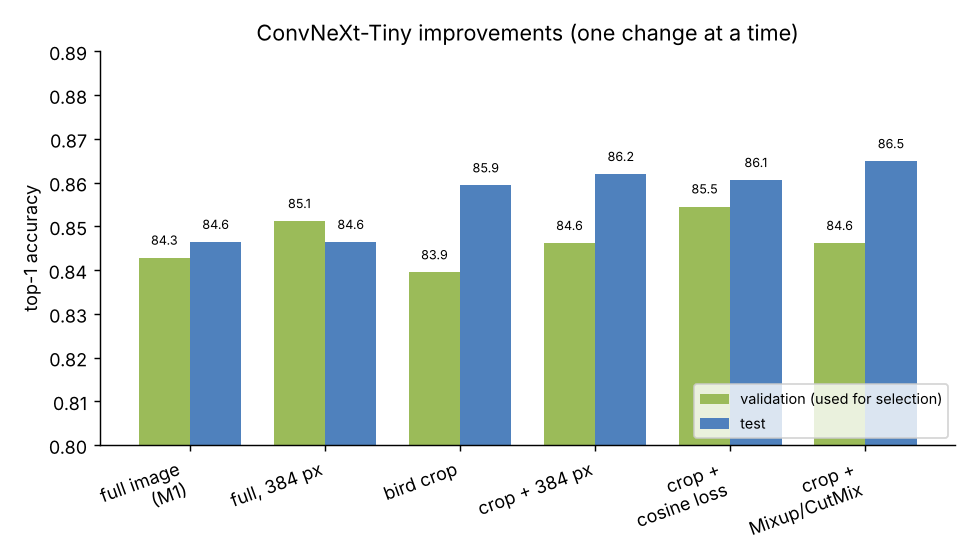
\includegraphics[width=0.85\linewidth]{figs/improve_convnext.png}
\caption{ConvNeXt-Tiny: one change at a time (validation and test accuracy).}
\end{figure}

\begin{table}[H]\centering\small
\begin{tabular}{lcccc}
\toprule
ConvNeXt-Tiny run & Val & Test & Test + TTA & Macro-F1\\
\midrule
Full image, 224\,px (Milestone-1 baseline) & 84.3 & 84.6 & --- & 84.5\\
Full image, 384\,px & 85.1 & 84.6 & 84.9 & 84.5\\
Bird crop, 224\,px & 83.9 & 85.9 & 86.3 & 85.8\\
Bird crop, 384\,px & 84.6 & 86.2 & 86.5 & 86.1\\
Bird crop, cosine loss & \textbf{85.5} & 86.1 & 86.5 & 86.0\\
Bird crop, Mixup/CutMix (40 ep.) & 84.6 & \textbf{86.5} & \textbf{86.7} & \textbf{86.4}\\
\bottomrule
\end{tabular}
\caption{ConvNeXt-Tiny improvements (\%). Validation differences below $\sim$1.5 points are within noise (598 images).}
\end{table}

%FINALRUNS
